\documentclass[a4paper]{article}

% Packages
\usepackage{listings}
\usepackage{color}
\usepackage[utf8]{inputenc}
\usepackage{listingsutf8}
\usepackage{graphicx}
\usepackage{epstopdf}
\usepackage{fancyhdr}
\usepackage[T1]{fontenc}
%\usepackage[top=2cm, bottom=2cm, left=3.5cm, right=2cm]{geometry} % Les marges.
\usepackage[top=2cm, bottom=2cm, left=2cm, right=2cm]{geometry} % Les marges.

\definecolor{mygreen}{rgb}{0,0.6,0}
\definecolor{mygray}{rgb}{0.5,0.5,0.5}
\definecolor{mymauve}{rgb}{0.58,0,0.82}
\definecolor{bggray}{rgb}{0.95, 0.95, 0.95}
\lstset{inputencoding=utf8/latin1}
\lstset{ %
    backgroundcolor=\color{bggray},   % choose the background color; you must add \usepackage{color} or \usepackage{xcolor}
    basicstyle=\footnotesize,        % the size of the fonts that are used for the code
    breakatwhitespace=false,         % sets if automatic breaks should only happen at whitespace
    breaklines=true,                 % sets automatic line breaking
    captionpos=b,                    % sets the caption-position to bottom
    commentstyle=\color{mygreen},    % comment style
    deletekeywords={...},            % if you want to delete keywords from the given language
    escapeinside={\%*}{*)},          % if you want to add LaTeX within your code
    extendedchars=true,              % lets you use non-ASCII characters; for 8-bits encodings only, does not work with UTF-8
    frame=single,                    % adds a frame around the code
    frameround=tttt                  % tttt for having the corner round.
    keepspaces=true,                 % keeps spaces in text, useful for keeping indentation of code (possibly needs columns=flexible)
    keywordstyle=\color{blue},       % keyword style
    language=Matlab,                 % the language of the code
    morekeywords={*,...},            % if you want to add more keywords to the set
    numbers=left,                    % where to put the line-numbers; possible values are (none, left, right)
    numbersep=5pt,                   % how far the line-numbers are from the code
    numberstyle=\tiny\color{mygray}, % the style that is used for the line-numbers
    rulecolor=\color{black},         % if not set, the frame-color may be changed on line-breaks within not-black text (e.g. comments (green here))
    showspaces=false,                % show spaces everywhere adding particular underscores; it overrides 'showstringspaces'
    showstringspaces=false,          % underline spaces within strings only
    showtabs=false,                  % show tabs within strings adding particular underscores
    stepnumber=1,                    % the step between two line-numbers. If it's 1, each line will be numbered
    stringstyle=\color{mymauve},     % string literal style
    tabsize=2,                       % sets default tabsize to 2 spaces
    title=\lstname                   % show the filename of files included with \lstinputlisting; also try caption instead of title
}

% Header
\pagestyle{fancy}
\fancyhead[L]{Axel Fahy \& Rudolf Höhn}
\fancyhead[R]{\today}

\title{TP Design Patterns\\Conception orientée objet}
\author{Axel Fahy \& Rudolf Höhn}
\date{\today}

\begin{document}
\maketitle

\section{Contexte de développement}
Pour ce travail pratique, nous avons choisi le jeu du Sudoku.
L'utilisateur peut jouer au Sudoku suivant les règles standardes pour une grille 9x9.
Le jeu se fait en ligne de commande, à chaque tour, on demande à l'utilisateur s'il veut continuer ou arrêter le jeu,
s'il veut utiliser un code de triche ou revenir dans un état précédent et dans quelle case veut-il placer le nouveau numéro.
\\\\
Pour la partie triche et mémoire du jeu, nous avons utilisé les Design Pattern Adapter et Memento.

\section{Description des Design Patterns}

\subsection{Memento}
Le Design Pattern Memento nous sert à mémoriser les précédents états du jeu, c'est-à-dire, des états de notre \textit{Sudoku}.
Dans la classe \textit{SudokuGame}, nous avons une liste de \textit{Memento} où chaque instance sera un état du jeu, et un objet \textit{Originator} qui connaitra l'état actuel du jeu.
Seul l'\textit{Originator} peut aller lire ou modifier un état du jeu, soit un \textit{Memento}.\\\\
Si l'utilisateur décide de revenir à un état précédent, il pourra revenir d'autant de coups qu'il veut, et s'il est allé trop en arrière, il pourra revenir dans le temps (retour vers le futur, mais sans Dolorean).
\begin{center}
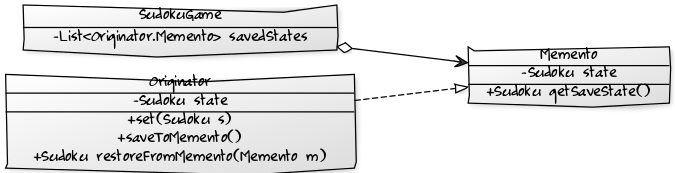
\includegraphics[scale=0.7]{../diagrams/memento.png}
\end{center}
Ce Design Pattern apporte une gestion des états très simple à mettre en œuvre.
Le \textit{Memento} est une classe opaque au jeu (ou \textit{Caretaker} dans la littérature), et c'est pour garder le principe d'encapsulation qu'on passe par l'\textit{Originator}.
\newpage
\subsection{Adapter}
Le Design Adapter nous permet d'utiliser une fonction/algorithme provenant d'une autre classe sans devoir adapter notre code ou le code de l'algorithme pour se conformer à notre implémentation.
Dans notre cas, nous avions à disposition un résolveur de Sudoku, \textit{SudoKiller} qui, à partir d'un \textit{SudokuBoard}, résoud le Sudoku.
Nous avons donc pour cela implémenté une classe \textit{SudokuSolverAdapter} qui reçoit un objet \textit{Sudoku}, extrait la grille, crée un objet \textit{SudokuBoard} et appelle une instance de \textit{CustomKiller} pour trouver la bonne réponse.
La classe \textit{SudoKiller} étant abstraite, nous avons du définir une classe qui l'étend.
\begin{center}
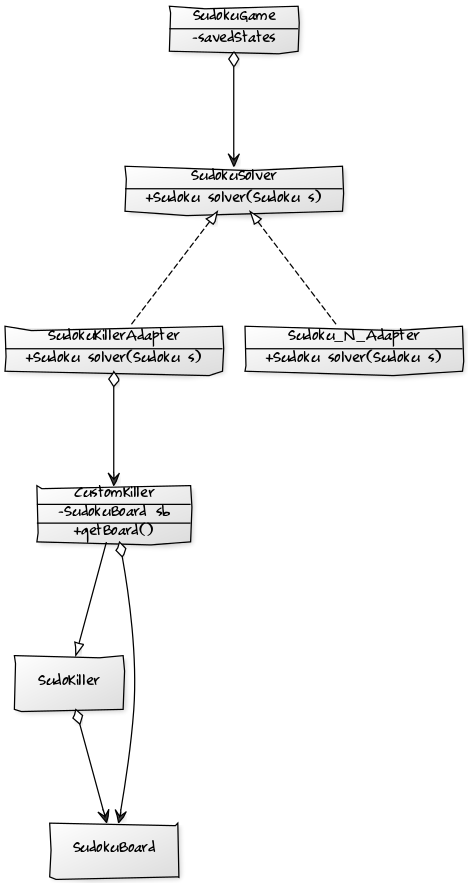
\includegraphics[scale=0.7]{../diagrams/adapter.png}
\end{center}
Ce Design Pattern nous permettrait de, par exemple, utiliser d'autres algorithmes de résolution de Sudoku sans devoir changer notre code de jeu, il faudrait juste rajouter une fonction \textit{solverOther} où 'Other' serait l'autre algorithme.
On comprend donc assez bien son utilité, elle permet de construire un lien entre deux programmes différents pour augmenter les capacités du premier.
\newpage
\section{Discussion}

\section{TODO}
Taille du tableau de board est 9 en dur dans le code

\end{document}
